\documentclass[twoside]{book}

% Packages required by doxygen
\usepackage{fixltx2e}
\usepackage{calc}
\usepackage{doxygen}
\usepackage[export]{adjustbox} % also loads graphicx
\usepackage{graphicx}
\usepackage[utf8]{inputenc}
\usepackage{makeidx}
\usepackage{multicol}
\usepackage{multirow}
\PassOptionsToPackage{warn}{textcomp}
\usepackage{textcomp}
\usepackage[nointegrals]{wasysym}
\usepackage[table]{xcolor}

% Font selection
\usepackage[T1]{fontenc}
\usepackage[scaled=.90]{helvet}
\usepackage{courier}
\usepackage{amssymb}
\usepackage{sectsty}
\renewcommand{\familydefault}{\sfdefault}
\allsectionsfont{%
  \fontseries{bc}\selectfont%
  \color{darkgray}%
}
\renewcommand{\DoxyLabelFont}{%
  \fontseries{bc}\selectfont%
  \color{darkgray}%
}
\newcommand{\+}{\discretionary{\mbox{\scriptsize$\hookleftarrow$}}{}{}}

% Page & text layout
\usepackage{geometry}
\geometry{%
  a4paper,%
  top=2.5cm,%
  bottom=2.5cm,%
  left=2.5cm,%
  right=2.5cm%
}
\tolerance=750
\hfuzz=15pt
\hbadness=750
\setlength{\emergencystretch}{15pt}
\setlength{\parindent}{0cm}
\setlength{\parskip}{3ex plus 2ex minus 2ex}
\makeatletter
\renewcommand{\paragraph}{%
  \@startsection{paragraph}{4}{0ex}{-1.0ex}{1.0ex}{%
    \normalfont\normalsize\bfseries\SS@parafont%
  }%
}
\renewcommand{\subparagraph}{%
  \@startsection{subparagraph}{5}{0ex}{-1.0ex}{1.0ex}{%
    \normalfont\normalsize\bfseries\SS@subparafont%
  }%
}
\makeatother

% Headers & footers
\usepackage{fancyhdr}
\pagestyle{fancyplain}
\fancyhead[LE]{\fancyplain{}{\bfseries\thepage}}
\fancyhead[CE]{\fancyplain{}{}}
\fancyhead[RE]{\fancyplain{}{\bfseries\leftmark}}
\fancyhead[LO]{\fancyplain{}{\bfseries\rightmark}}
\fancyhead[CO]{\fancyplain{}{}}
\fancyhead[RO]{\fancyplain{}{\bfseries\thepage}}
\fancyfoot[LE]{\fancyplain{}{}}
\fancyfoot[CE]{\fancyplain{}{}}
\fancyfoot[RE]{\fancyplain{}{\bfseries\scriptsize Generated by Doxygen }}
\fancyfoot[LO]{\fancyplain{}{\bfseries\scriptsize Generated by Doxygen }}
\fancyfoot[CO]{\fancyplain{}{}}
\fancyfoot[RO]{\fancyplain{}{}}
\renewcommand{\footrulewidth}{0.4pt}
\renewcommand{\chaptermark}[1]{%
  \markboth{#1}{}%
}
\renewcommand{\sectionmark}[1]{%
  \markright{\thesection\ #1}%
}

% Indices & bibliography
\usepackage{natbib}
\usepackage[titles]{tocloft}
\setcounter{tocdepth}{3}
\setcounter{secnumdepth}{5}
\makeindex

% Hyperlinks (required, but should be loaded last)
\usepackage{ifpdf}
\ifpdf
  \usepackage[pdftex,pagebackref=true]{hyperref}
\else
  \usepackage[ps2pdf,pagebackref=true]{hyperref}
\fi
\hypersetup{%
  colorlinks=true,%
  linkcolor=blue,%
  citecolor=blue,%
  unicode%
}

% Custom commands
\newcommand{\clearemptydoublepage}{%
  \newpage{\pagestyle{empty}\cleardoublepage}%
}

\usepackage{caption}
\captionsetup{labelsep=space,justification=centering,font={bf},singlelinecheck=off,skip=4pt,position=top}

%===== C O N T E N T S =====

\begin{document}

% Titlepage & ToC
\hypersetup{pageanchor=false,
             bookmarksnumbered=true,
             pdfencoding=unicode
            }
\pagenumbering{alph}
\begin{titlepage}
\vspace*{7cm}
\begin{center}%
{\Large Projeto 1 }\\
\vspace*{1cm}
{\large Generated by Doxygen 1.8.14}\\
\end{center}
\end{titlepage}
\clearemptydoublepage
\pagenumbering{roman}
\tableofcontents
\clearemptydoublepage
\pagenumbering{arabic}
\hypersetup{pageanchor=true}

%--- Begin generated contents ---
\chapter{Hierarchical Index}
\section{Class Hierarchy}
This inheritance list is sorted roughly, but not completely, alphabetically\+:\begin{DoxyCompactList}
\item \contentsline{section}{Poligono}{\pageref{class_poligono}}{}
\begin{DoxyCompactList}
\item \contentsline{section}{Retangulo}{\pageref{class_retangulo}}{}
\end{DoxyCompactList}
\item \contentsline{section}{Ponto}{\pageref{class_ponto}}{}
\end{DoxyCompactList}

\chapter{Class Index}
\section{Class List}
Here are the classes, structs, unions and interfaces with brief descriptions\+:\begin{DoxyCompactList}
\item\contentsline{section}{\mbox{\hyperlink{class_poligono}{Poligono}} }{\pageref{class_poligono}}{}
\item\contentsline{section}{\mbox{\hyperlink{class_ponto}{Ponto}} }{\pageref{class_ponto}}{}
\item\contentsline{section}{\mbox{\hyperlink{class_retangulo}{Retangulo}} }{\pageref{class_retangulo}}{}
\end{DoxyCompactList}

\chapter{File Index}
\section{File List}
Here is a list of all files with brief descriptions\+:\begin{DoxyCompactList}
\item\contentsline{section}{C\+:/\+Users/\+Adamstor Pequeno/\+Documents/\+Projeto1/\mbox{\hyperlink{main_8cpp}{main.\+cpp}} }{\pageref{main_8cpp}}{}
\item\contentsline{section}{C\+:/\+Users/\+Adamstor Pequeno/\+Documents/\+Projeto1/\mbox{\hyperlink{poligono_8cpp}{poligono.\+cpp}} }{\pageref{poligono_8cpp}}{}
\item\contentsline{section}{C\+:/\+Users/\+Adamstor Pequeno/\+Documents/\+Projeto1/\mbox{\hyperlink{poligono_8h}{poligono.\+h}} }{\pageref{poligono_8h}}{}
\item\contentsline{section}{C\+:/\+Users/\+Adamstor Pequeno/\+Documents/\+Projeto1/\mbox{\hyperlink{ponto_8cpp}{ponto.\+cpp}} }{\pageref{ponto_8cpp}}{}
\item\contentsline{section}{C\+:/\+Users/\+Adamstor Pequeno/\+Documents/\+Projeto1/\mbox{\hyperlink{ponto_8h}{ponto.\+h}} }{\pageref{ponto_8h}}{}
\item\contentsline{section}{C\+:/\+Users/\+Adamstor Pequeno/\+Documents/\+Projeto1/\mbox{\hyperlink{retangulo_8cpp}{retangulo.\+cpp}} }{\pageref{retangulo_8cpp}}{}
\item\contentsline{section}{C\+:/\+Users/\+Adamstor Pequeno/\+Documents/\+Projeto1/\mbox{\hyperlink{retangulo_8h}{retangulo.\+h}} }{\pageref{retangulo_8h}}{}
\end{DoxyCompactList}

\chapter{Class Documentation}
\hypertarget{class_poligono}{}\section{Poligono Class Reference}
\label{class_poligono}\index{Poligono@{Poligono}}


{\ttfamily \#include $<$poligono.\+h$>$}

Inheritance diagram for Poligono\+:\begin{figure}[H]
\begin{center}
\leavevmode
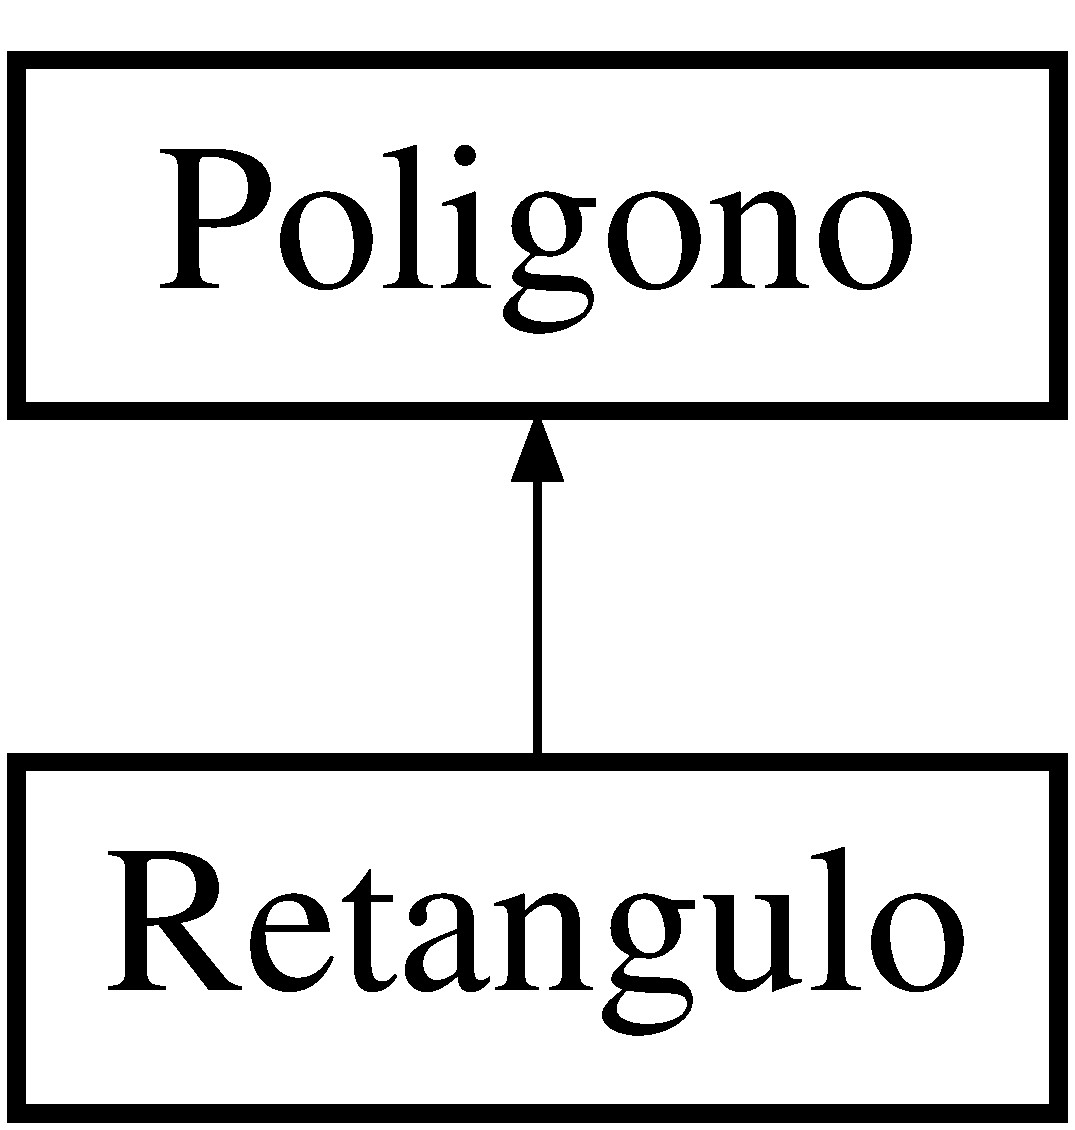
\includegraphics[height=2.000000cm]{class_poligono}
\end{center}
\end{figure}
\subsection*{Public Member Functions}
\begin{DoxyCompactItemize}
\item 
\mbox{\hyperlink{class_poligono_a9311a9a1496878c09c8508b3636e2870}{Poligono}} ()
\item 
int \mbox{\hyperlink{class_poligono_a345539e8cc714d4e429c92fbfbb825d6}{Contador}} ()
\begin{DoxyCompactList}\small\item\em Um contador básico. \end{DoxyCompactList}\item 
int \mbox{\hyperlink{class_poligono_a0e4a1dda914bb96506976c0ff2f17f23}{vertices}} ()
\begin{DoxyCompactList}\small\item\em Retorna o numero de vertices. \end{DoxyCompactList}\item 
void \mbox{\hyperlink{class_poligono_ae1be40b54bc95099e1296e156b246881}{Add\+Vert}} (\mbox{\hyperlink{class_ponto}{Ponto}} \+\_\+x)
\begin{DoxyCompactList}\small\item\em Adiciona vertice. \end{DoxyCompactList}\item 
void \mbox{\hyperlink{class_poligono_ac22d76a087d08ea82627be416404ae15}{print}} ()
\begin{DoxyCompactList}\small\item\em Imprime os pontos dos vertices. \end{DoxyCompactList}\item 
float \mbox{\hyperlink{class_poligono_a15cc3e743e4347d966ba12fa2cdb69b7}{Area}} ()
\begin{DoxyCompactList}\small\item\em Retorna a area do poligono. \end{DoxyCompactList}\item 
void \mbox{\hyperlink{class_poligono_aafacd43b0918e0765fbb42d9aad5bb35}{translada}} (float \+\_\+a, float \+\_\+b)
\begin{DoxyCompactList}\small\item\em translada o poligono de +a e +b. \end{DoxyCompactList}\item 
void \mbox{\hyperlink{class_poligono_a487911a74fc40ea3cdea61380889e180}{rotacao}} (float teta, float x0, float y0)
\begin{DoxyCompactList}\small\item\em rotaciona o poligono \end{DoxyCompactList}\end{DoxyCompactItemize}


\subsection{Constructor \& Destructor Documentation}
\mbox{\Hypertarget{class_poligono_a9311a9a1496878c09c8508b3636e2870}\label{class_poligono_a9311a9a1496878c09c8508b3636e2870}} 
\index{Poligono@{Poligono}!Poligono@{Poligono}}
\index{Poligono@{Poligono}!Poligono@{Poligono}}
\subsubsection{\texorpdfstring{Poligono()}{Poligono()}}
{\footnotesize\ttfamily Poligono\+::\+Poligono (\begin{DoxyParamCaption}{ }\end{DoxyParamCaption})}



\subsection{Member Function Documentation}
\mbox{\Hypertarget{class_poligono_ae1be40b54bc95099e1296e156b246881}\label{class_poligono_ae1be40b54bc95099e1296e156b246881}} 
\index{Poligono@{Poligono}!Add\+Vert@{Add\+Vert}}
\index{Add\+Vert@{Add\+Vert}!Poligono@{Poligono}}
\subsubsection{\texorpdfstring{Add\+Vert()}{AddVert()}}
{\footnotesize\ttfamily void Poligono\+::\+Add\+Vert (\begin{DoxyParamCaption}\item[{\mbox{\hyperlink{class_ponto}{Ponto}}}]{\+\_\+x }\end{DoxyParamCaption})}



Adiciona vertice. 

A função adiciona adiciona um vertice no ponto dado como argumento, e soma +1 no contador. \mbox{\Hypertarget{class_poligono_a15cc3e743e4347d966ba12fa2cdb69b7}\label{class_poligono_a15cc3e743e4347d966ba12fa2cdb69b7}} 
\index{Poligono@{Poligono}!Area@{Area}}
\index{Area@{Area}!Poligono@{Poligono}}
\subsubsection{\texorpdfstring{Area()}{Area()}}
{\footnotesize\ttfamily float Poligono\+::\+Area (\begin{DoxyParamCaption}{ }\end{DoxyParamCaption})}



Retorna a area do poligono. 

Retorna a area do poligono usando somas e subtracoes. \mbox{\Hypertarget{class_poligono_a345539e8cc714d4e429c92fbfbb825d6}\label{class_poligono_a345539e8cc714d4e429c92fbfbb825d6}} 
\index{Poligono@{Poligono}!Contador@{Contador}}
\index{Contador@{Contador}!Poligono@{Poligono}}
\subsubsection{\texorpdfstring{Contador()}{Contador()}}
{\footnotesize\ttfamily int Poligono\+::\+Contador (\begin{DoxyParamCaption}{ }\end{DoxyParamCaption})}



Um contador básico. 

Contador utilizado para contar o numero de vertices \mbox{\Hypertarget{class_poligono_ac22d76a087d08ea82627be416404ae15}\label{class_poligono_ac22d76a087d08ea82627be416404ae15}} 
\index{Poligono@{Poligono}!print@{print}}
\index{print@{print}!Poligono@{Poligono}}
\subsubsection{\texorpdfstring{print()}{print()}}
{\footnotesize\ttfamily void Poligono\+::print (\begin{DoxyParamCaption}{ }\end{DoxyParamCaption})}



Imprime os pontos dos vertices. 

Imprime cada um dos vertices do poligono no formato (x,y)-\/$>$(a,b). \mbox{\Hypertarget{class_poligono_a487911a74fc40ea3cdea61380889e180}\label{class_poligono_a487911a74fc40ea3cdea61380889e180}} 
\index{Poligono@{Poligono}!rotacao@{rotacao}}
\index{rotacao@{rotacao}!Poligono@{Poligono}}
\subsubsection{\texorpdfstring{rotacao()}{rotacao()}}
{\footnotesize\ttfamily void Poligono\+::rotacao (\begin{DoxyParamCaption}\item[{float}]{teta,  }\item[{float}]{x0,  }\item[{float}]{y0 }\end{DoxyParamCaption})}



rotaciona o poligono 

rotaciona o poligono de um angulo dado como argumento. \mbox{\Hypertarget{class_poligono_aafacd43b0918e0765fbb42d9aad5bb35}\label{class_poligono_aafacd43b0918e0765fbb42d9aad5bb35}} 
\index{Poligono@{Poligono}!translada@{translada}}
\index{translada@{translada}!Poligono@{Poligono}}
\subsubsection{\texorpdfstring{translada()}{translada()}}
{\footnotesize\ttfamily void Poligono\+::translada (\begin{DoxyParamCaption}\item[{float}]{\+\_\+a,  }\item[{float}]{\+\_\+b }\end{DoxyParamCaption})}



translada o poligono de +a e +b. 

Soma os argumentos \+\_\+a e \+\_\+b nos valores do poligono, alterando sua localizacao \mbox{\Hypertarget{class_poligono_a0e4a1dda914bb96506976c0ff2f17f23}\label{class_poligono_a0e4a1dda914bb96506976c0ff2f17f23}} 
\index{Poligono@{Poligono}!vertices@{vertices}}
\index{vertices@{vertices}!Poligono@{Poligono}}
\subsubsection{\texorpdfstring{vertices()}{vertices()}}
{\footnotesize\ttfamily int Poligono\+::vertices (\begin{DoxyParamCaption}{ }\end{DoxyParamCaption})}



Retorna o numero de vertices. 

Retorna o valor do contador de vertices 

The documentation for this class was generated from the following files\+:\begin{DoxyCompactItemize}
\item 
C\+:/\+Users/\+Adamstor Pequeno/\+Documents/\+Projeto1/\mbox{\hyperlink{poligono_8h}{poligono.\+h}}\item 
C\+:/\+Users/\+Adamstor Pequeno/\+Documents/\+Projeto1/\mbox{\hyperlink{poligono_8cpp}{poligono.\+cpp}}\end{DoxyCompactItemize}

\hypertarget{class_ponto}{}\section{Ponto Class Reference}
\label{class_ponto}\index{Ponto@{Ponto}}


{\ttfamily \#include $<$ponto.\+h$>$}

\subsection*{Public Member Functions}
\begin{DoxyCompactItemize}
\item 
\mbox{\hyperlink{class_ponto_a49b03b00e9ebc01c2011c25f6517b93b}{Ponto}} ()
\begin{DoxyCompactList}\small\item\em Construtor Padrão. \end{DoxyCompactList}\item 
\mbox{\hyperlink{class_ponto_a150e330b2856e42528c4521d575f9179}{Ponto}} (float \+\_\+x, float \+\_\+y)
\begin{DoxyCompactList}\small\item\em Construtor com Argumentos. \end{DoxyCompactList}\item 
void \mbox{\hyperlink{class_ponto_a3dcee3a98a8863d4067a8de537b2a433}{print}} ()
\begin{DoxyCompactList}\small\item\em Imprime o ponto na tela. \end{DoxyCompactList}\item 
void \mbox{\hyperlink{class_ponto_a22129ad4dbf8019c479021d70a9f6774}{setX}} (float \+\_\+x)
\begin{DoxyCompactList}\small\item\em Define o valor de X. \end{DoxyCompactList}\item 
void \mbox{\hyperlink{class_ponto_a2d9e5b9fade9d3f3f21122a2dc2f5e11}{setY}} (float \+\_\+y)
\begin{DoxyCompactList}\small\item\em Define o valor de Y. \end{DoxyCompactList}\item 
void \mbox{\hyperlink{class_ponto_a827488219a7da184d440f687cec49ce6}{set\+XY}} (float \+\_\+x, float \+\_\+y)
\begin{DoxyCompactList}\small\item\em Define os valores de X e Y. \end{DoxyCompactList}\item 
float \mbox{\hyperlink{class_ponto_ae4823d6ee26ff3448ee403d26a3c6d2f}{getX}} ()
\begin{DoxyCompactList}\small\item\em Retorna o valor de X. \end{DoxyCompactList}\item 
float \mbox{\hyperlink{class_ponto_ab120600953e6544301223b9b05a43ee5}{getY}} ()
\begin{DoxyCompactList}\small\item\em Retorna o valor de Y. \end{DoxyCompactList}\item 
\mbox{\hyperlink{class_ponto}{Ponto}} \mbox{\hyperlink{class_ponto_ab53f257f937ed29a7ed5a1051014773f}{add}} (\mbox{\hyperlink{class_ponto}{Ponto}} \+\_\+p)
\begin{DoxyCompactList}\small\item\em Soma dois pontos. \end{DoxyCompactList}\item 
\mbox{\hyperlink{class_ponto}{Ponto}} \mbox{\hyperlink{class_ponto_a4c49d0e1863d645a6a8ac68c823b23bb}{sub}} (\mbox{\hyperlink{class_ponto}{Ponto}} \+\_\+p)
\begin{DoxyCompactList}\small\item\em Subtrai dois pontos. \end{DoxyCompactList}\item 
double \mbox{\hyperlink{class_ponto_aabf21d159fc5b233d5e58d06cc4a6b6c}{norma}} ()
\begin{DoxyCompactList}\small\item\em Calcula a norma do ponto. \end{DoxyCompactList}\item 
\mbox{\hyperlink{class_ponto}{Ponto}} \mbox{\hyperlink{class_ponto_a7e481afed576885a03c7a3db34df29fa}{translada}} (float \+\_\+x, float \+\_\+y)
\begin{DoxyCompactList}\small\item\em translada o ponto em +x e +y \end{DoxyCompactList}\end{DoxyCompactItemize}


\subsection{Constructor \& Destructor Documentation}
\mbox{\Hypertarget{class_ponto_a49b03b00e9ebc01c2011c25f6517b93b}\label{class_ponto_a49b03b00e9ebc01c2011c25f6517b93b}} 
\index{Ponto@{Ponto}!Ponto@{Ponto}}
\index{Ponto@{Ponto}!Ponto@{Ponto}}
\subsubsection{\texorpdfstring{Ponto()}{Ponto()}\hspace{0.1cm}{\footnotesize\ttfamily [1/2]}}
{\footnotesize\ttfamily Ponto\+::\+Ponto (\begin{DoxyParamCaption}{ }\end{DoxyParamCaption})}



Construtor Padrão. 

Construtor Padrão que define os valores das variáveis x e y como 0. \mbox{\Hypertarget{class_ponto_a150e330b2856e42528c4521d575f9179}\label{class_ponto_a150e330b2856e42528c4521d575f9179}} 
\index{Ponto@{Ponto}!Ponto@{Ponto}}
\index{Ponto@{Ponto}!Ponto@{Ponto}}
\subsubsection{\texorpdfstring{Ponto()}{Ponto()}\hspace{0.1cm}{\footnotesize\ttfamily [2/2]}}
{\footnotesize\ttfamily Ponto\+::\+Ponto (\begin{DoxyParamCaption}\item[{float}]{\+\_\+x,  }\item[{float}]{\+\_\+y }\end{DoxyParamCaption})}



Construtor com Argumentos. 

Construtor com Argumentos que define os valores de acordo com o input do usuário. 

\subsection{Member Function Documentation}
\mbox{\Hypertarget{class_ponto_ab53f257f937ed29a7ed5a1051014773f}\label{class_ponto_ab53f257f937ed29a7ed5a1051014773f}} 
\index{Ponto@{Ponto}!add@{add}}
\index{add@{add}!Ponto@{Ponto}}
\subsubsection{\texorpdfstring{add()}{add()}}
{\footnotesize\ttfamily \mbox{\hyperlink{class_ponto}{Ponto}} Ponto\+::add (\begin{DoxyParamCaption}\item[{\mbox{\hyperlink{class_ponto}{Ponto}}}]{\+\_\+p }\end{DoxyParamCaption})}



Soma dois pontos. 

Função usada para somar o valor de dois pontos, usando um ponto como input da função \mbox{\Hypertarget{class_ponto_ae4823d6ee26ff3448ee403d26a3c6d2f}\label{class_ponto_ae4823d6ee26ff3448ee403d26a3c6d2f}} 
\index{Ponto@{Ponto}!getX@{getX}}
\index{getX@{getX}!Ponto@{Ponto}}
\subsubsection{\texorpdfstring{get\+X()}{getX()}}
{\footnotesize\ttfamily float Ponto\+::getX (\begin{DoxyParamCaption}{ }\end{DoxyParamCaption})}



Retorna o valor de X. 

Função usada para obter o valor de X \mbox{\Hypertarget{class_ponto_ab120600953e6544301223b9b05a43ee5}\label{class_ponto_ab120600953e6544301223b9b05a43ee5}} 
\index{Ponto@{Ponto}!getY@{getY}}
\index{getY@{getY}!Ponto@{Ponto}}
\subsubsection{\texorpdfstring{get\+Y()}{getY()}}
{\footnotesize\ttfamily float Ponto\+::getY (\begin{DoxyParamCaption}{ }\end{DoxyParamCaption})}



Retorna o valor de Y. 

Função usada para obter o valor de Y \mbox{\Hypertarget{class_ponto_aabf21d159fc5b233d5e58d06cc4a6b6c}\label{class_ponto_aabf21d159fc5b233d5e58d06cc4a6b6c}} 
\index{Ponto@{Ponto}!norma@{norma}}
\index{norma@{norma}!Ponto@{Ponto}}
\subsubsection{\texorpdfstring{norma()}{norma()}}
{\footnotesize\ttfamily double Ponto\+::norma (\begin{DoxyParamCaption}{ }\end{DoxyParamCaption})}



Calcula a norma do ponto. 

Retorna a norma do ponto. \mbox{\Hypertarget{class_ponto_a3dcee3a98a8863d4067a8de537b2a433}\label{class_ponto_a3dcee3a98a8863d4067a8de537b2a433}} 
\index{Ponto@{Ponto}!print@{print}}
\index{print@{print}!Ponto@{Ponto}}
\subsubsection{\texorpdfstring{print()}{print()}}
{\footnotesize\ttfamily void Ponto\+::print (\begin{DoxyParamCaption}{ }\end{DoxyParamCaption})}



Imprime o ponto na tela. 

Usando o console, imprime o ponto na tela no formato (x,y). \mbox{\Hypertarget{class_ponto_a22129ad4dbf8019c479021d70a9f6774}\label{class_ponto_a22129ad4dbf8019c479021d70a9f6774}} 
\index{Ponto@{Ponto}!setX@{setX}}
\index{setX@{setX}!Ponto@{Ponto}}
\subsubsection{\texorpdfstring{set\+X()}{setX()}}
{\footnotesize\ttfamily void Ponto\+::setX (\begin{DoxyParamCaption}\item[{float}]{\+\_\+x }\end{DoxyParamCaption})}



Define o valor de X. 

Pelo input do usuário, define o valor X do objeto \mbox{\hyperlink{class_ponto}{Ponto}}. \mbox{\Hypertarget{class_ponto_a827488219a7da184d440f687cec49ce6}\label{class_ponto_a827488219a7da184d440f687cec49ce6}} 
\index{Ponto@{Ponto}!set\+XY@{set\+XY}}
\index{set\+XY@{set\+XY}!Ponto@{Ponto}}
\subsubsection{\texorpdfstring{set\+X\+Y()}{setXY()}}
{\footnotesize\ttfamily void Ponto\+::set\+XY (\begin{DoxyParamCaption}\item[{float}]{\+\_\+x,  }\item[{float}]{\+\_\+y }\end{DoxyParamCaption})}



Define os valores de X e Y. 

Pelo input do usuário, define os valores X e Y do objeto \mbox{\hyperlink{class_ponto}{Ponto}}. \mbox{\Hypertarget{class_ponto_a2d9e5b9fade9d3f3f21122a2dc2f5e11}\label{class_ponto_a2d9e5b9fade9d3f3f21122a2dc2f5e11}} 
\index{Ponto@{Ponto}!setY@{setY}}
\index{setY@{setY}!Ponto@{Ponto}}
\subsubsection{\texorpdfstring{set\+Y()}{setY()}}
{\footnotesize\ttfamily void Ponto\+::setY (\begin{DoxyParamCaption}\item[{float}]{\+\_\+y }\end{DoxyParamCaption})}



Define o valor de Y. 

Pelo input do usuário, define o valor Y do objeto \mbox{\hyperlink{class_ponto}{Ponto}}. \mbox{\Hypertarget{class_ponto_a4c49d0e1863d645a6a8ac68c823b23bb}\label{class_ponto_a4c49d0e1863d645a6a8ac68c823b23bb}} 
\index{Ponto@{Ponto}!sub@{sub}}
\index{sub@{sub}!Ponto@{Ponto}}
\subsubsection{\texorpdfstring{sub()}{sub()}}
{\footnotesize\ttfamily \mbox{\hyperlink{class_ponto}{Ponto}} Ponto\+::sub (\begin{DoxyParamCaption}\item[{\mbox{\hyperlink{class_ponto}{Ponto}}}]{\+\_\+p }\end{DoxyParamCaption})}



Subtrai dois pontos. 

Função usada para subtrair o valor de dois pontos, usando um ponto como argumento \mbox{\Hypertarget{class_ponto_a7e481afed576885a03c7a3db34df29fa}\label{class_ponto_a7e481afed576885a03c7a3db34df29fa}} 
\index{Ponto@{Ponto}!translada@{translada}}
\index{translada@{translada}!Ponto@{Ponto}}
\subsubsection{\texorpdfstring{translada()}{translada()}}
{\footnotesize\ttfamily \mbox{\hyperlink{class_ponto}{Ponto}} Ponto\+::translada (\begin{DoxyParamCaption}\item[{float}]{\+\_\+x,  }\item[{float}]{\+\_\+y }\end{DoxyParamCaption})}



translada o ponto em +x e +y 

Recebe dois valores como argumento e translada o ponto de acordo com eles 

The documentation for this class was generated from the following files\+:\begin{DoxyCompactItemize}
\item 
C\+:/\+Users/\+Adamstor Pequeno/\+Documents/\+Projeto1/\mbox{\hyperlink{ponto_8h}{ponto.\+h}}\item 
C\+:/\+Users/\+Adamstor Pequeno/\+Documents/\+Projeto1/\mbox{\hyperlink{ponto_8cpp}{ponto.\+cpp}}\end{DoxyCompactItemize}

\hypertarget{class_retangulo}{}\section{Retangulo Class Reference}
\label{class_retangulo}\index{Retangulo@{Retangulo}}


{\ttfamily \#include $<$retangulo.\+h$>$}

Inheritance diagram for Retangulo\+:\begin{figure}[H]
\begin{center}
\leavevmode
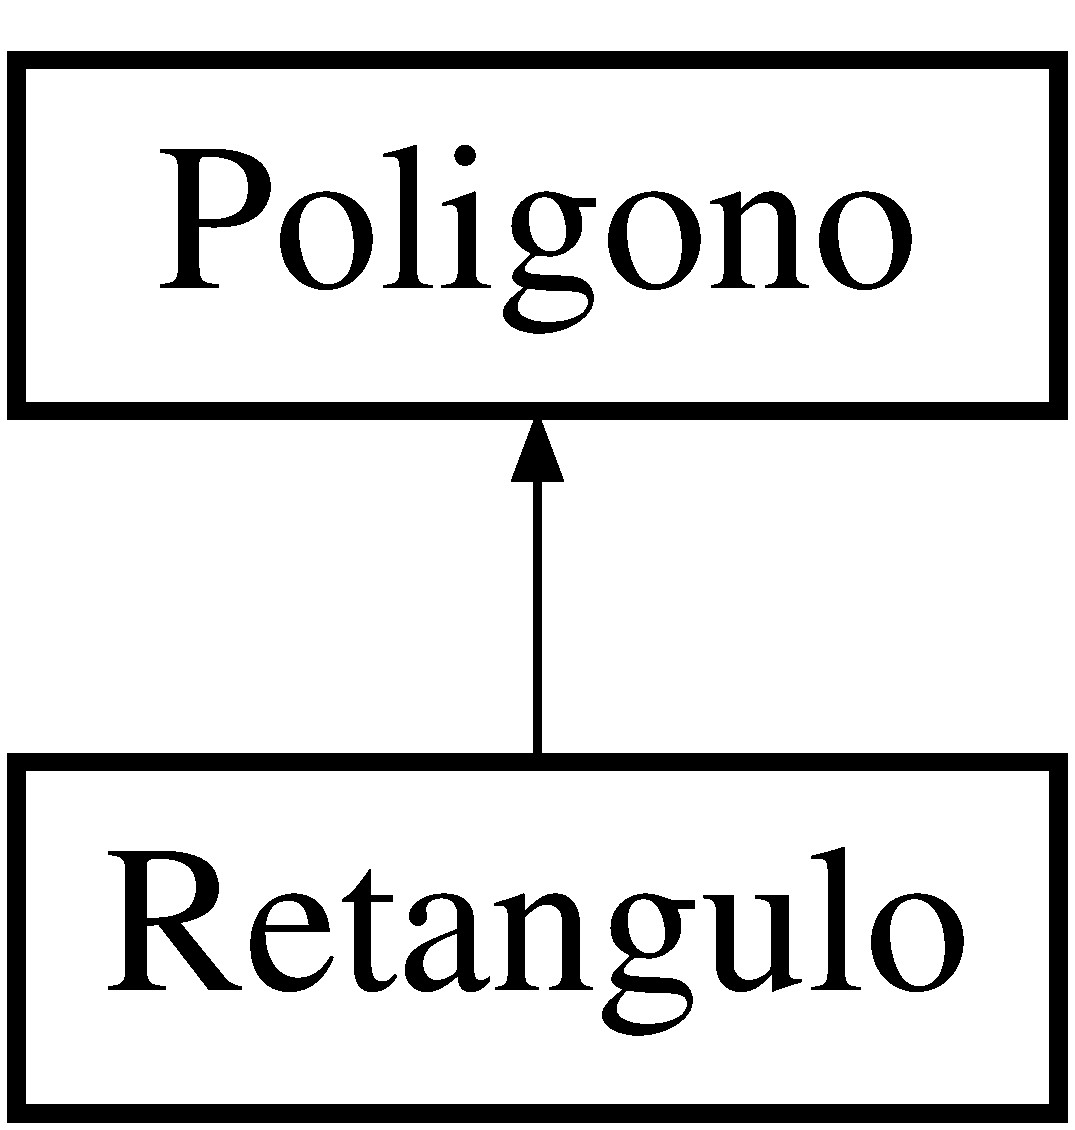
\includegraphics[height=2.000000cm]{class_retangulo}
\end{center}
\end{figure}
\subsection*{Public Member Functions}
\begin{DoxyCompactItemize}
\item 
\mbox{\hyperlink{class_retangulo_a54988c3e6af9f464d751940e32941d88}{Retangulo}} (float x, float y, float \+\_\+largura, float \+\_\+altura)
\begin{DoxyCompactList}\small\item\em Construtor da classe Retângulo. \end{DoxyCompactList}\end{DoxyCompactItemize}


\subsection{Constructor \& Destructor Documentation}
\mbox{\Hypertarget{class_retangulo_a54988c3e6af9f464d751940e32941d88}\label{class_retangulo_a54988c3e6af9f464d751940e32941d88}} 
\index{Retangulo@{Retangulo}!Retangulo@{Retangulo}}
\index{Retangulo@{Retangulo}!Retangulo@{Retangulo}}
\subsubsection{\texorpdfstring{Retangulo()}{Retangulo()}}
{\footnotesize\ttfamily Retangulo\+::\+Retangulo (\begin{DoxyParamCaption}\item[{float}]{x,  }\item[{float}]{y,  }\item[{float}]{\+\_\+largura,  }\item[{float}]{\+\_\+altura }\end{DoxyParamCaption})}



Construtor da classe Retângulo. 

Construtor com argumentos que utiliza as funções da classe Polígono para definir o retângulo a partir dos dados fornecidos. 

The documentation for this class was generated from the following files\+:\begin{DoxyCompactItemize}
\item 
C\+:/\+Users/\+Adamstor Pequeno/\+Documents/\+Projeto1/\mbox{\hyperlink{retangulo_8h}{retangulo.\+h}}\item 
C\+:/\+Users/\+Adamstor Pequeno/\+Documents/\+Projeto1/\mbox{\hyperlink{retangulo_8cpp}{retangulo.\+cpp}}\end{DoxyCompactItemize}

\chapter{File Documentation}
\hypertarget{main_8cpp}{}\section{C\+:/\+Users/\+Adamstor Pequeno/\+Documents/\+Projeto1/main.cpp File Reference}
\label{main_8cpp}\index{C\+:/\+Users/\+Adamstor Pequeno/\+Documents/\+Projeto1/main.\+cpp@{C\+:/\+Users/\+Adamstor Pequeno/\+Documents/\+Projeto1/main.\+cpp}}
{\ttfamily \#include $<$iostream$>$}\newline
{\ttfamily \#include \char`\"{}ponto.\+h\char`\"{}}\newline
{\ttfamily \#include \char`\"{}poligono.\+h\char`\"{}}\newline
\subsection*{Functions}
\begin{DoxyCompactItemize}
\item 
int \mbox{\hyperlink{main_8cpp_ae66f6b31b5ad750f1fe042a706a4e3d4}{main}} ()
\end{DoxyCompactItemize}


\subsection{Function Documentation}
\mbox{\Hypertarget{main_8cpp_ae66f6b31b5ad750f1fe042a706a4e3d4}\label{main_8cpp_ae66f6b31b5ad750f1fe042a706a4e3d4}} 
\index{main.\+cpp@{main.\+cpp}!main@{main}}
\index{main@{main}!main.\+cpp@{main.\+cpp}}
\subsubsection{\texorpdfstring{main()}{main()}}
{\footnotesize\ttfamily int main (\begin{DoxyParamCaption}{ }\end{DoxyParamCaption})}


\hypertarget{poligono_8cpp}{}\section{C\+:/\+Users/\+Adamstor Pequeno/\+Documents/\+Projeto1/poligono.cpp File Reference}
\label{poligono_8cpp}\index{C\+:/\+Users/\+Adamstor Pequeno/\+Documents/\+Projeto1/poligono.\+cpp@{C\+:/\+Users/\+Adamstor Pequeno/\+Documents/\+Projeto1/poligono.\+cpp}}
{\ttfamily \#include $<$iostream$>$}\newline
{\ttfamily \#include $<$cmath$>$}\newline
{\ttfamily \#include \char`\"{}poligono.\+h\char`\"{}}\newline
{\ttfamily \#include \char`\"{}ponto.\+h\char`\"{}}\newline
\subsection*{Macros}
\begin{DoxyCompactItemize}
\item 
\#define \mbox{\hyperlink{poligono_8cpp_a598a3330b3c21701223ee0ca14316eca}{PI}}~3.\+14159265
\end{DoxyCompactItemize}


\subsection{Macro Definition Documentation}
\mbox{\Hypertarget{poligono_8cpp_a598a3330b3c21701223ee0ca14316eca}\label{poligono_8cpp_a598a3330b3c21701223ee0ca14316eca}} 
\index{poligono.\+cpp@{poligono.\+cpp}!PI@{PI}}
\index{PI@{PI}!poligono.\+cpp@{poligono.\+cpp}}
\subsubsection{\texorpdfstring{PI}{PI}}
{\footnotesize\ttfamily \#define PI~3.\+14159265}


\hypertarget{poligono_8h}{}\section{C\+:/\+Users/\+Adamstor Pequeno/\+Documents/\+Projeto1/poligono.h File Reference}
\label{poligono_8h}\index{C\+:/\+Users/\+Adamstor Pequeno/\+Documents/\+Projeto1/poligono.\+h@{C\+:/\+Users/\+Adamstor Pequeno/\+Documents/\+Projeto1/poligono.\+h}}
{\ttfamily \#include \char`\"{}ponto.\+h\char`\"{}}\newline
\subsection*{Classes}
\begin{DoxyCompactItemize}
\item 
class \mbox{\hyperlink{class_poligono}{Poligono}}
\end{DoxyCompactItemize}

\hypertarget{ponto_8cpp}{}\section{C\+:/\+Users/\+Adamstor Pequeno/\+Documents/\+Projeto1/ponto.cpp File Reference}
\label{ponto_8cpp}\index{C\+:/\+Users/\+Adamstor Pequeno/\+Documents/\+Projeto1/ponto.\+cpp@{C\+:/\+Users/\+Adamstor Pequeno/\+Documents/\+Projeto1/ponto.\+cpp}}
{\ttfamily \#include $<$iostream$>$}\newline
{\ttfamily \#include $<$cmath$>$}\newline
{\ttfamily \#include \char`\"{}ponto.\+h\char`\"{}}\newline

\hypertarget{ponto_8h}{}\section{C\+:/\+Users/\+Adamstor Pequeno/\+Documents/\+Projeto1/ponto.h File Reference}
\label{ponto_8h}\index{C\+:/\+Users/\+Adamstor Pequeno/\+Documents/\+Projeto1/ponto.\+h@{C\+:/\+Users/\+Adamstor Pequeno/\+Documents/\+Projeto1/ponto.\+h}}
\subsection*{Classes}
\begin{DoxyCompactItemize}
\item 
class \mbox{\hyperlink{class_ponto}{Ponto}}
\end{DoxyCompactItemize}

\hypertarget{retangulo_8cpp}{}\section{C\+:/\+Users/\+Adamstor Pequeno/\+Documents/\+Projeto1/retangulo.cpp File Reference}
\label{retangulo_8cpp}\index{C\+:/\+Users/\+Adamstor Pequeno/\+Documents/\+Projeto1/retangulo.\+cpp@{C\+:/\+Users/\+Adamstor Pequeno/\+Documents/\+Projeto1/retangulo.\+cpp}}
{\ttfamily \#include $<$iostream$>$}\newline
{\ttfamily \#include \char`\"{}poligono.\+h\char`\"{}}\newline
{\ttfamily \#include \char`\"{}ponto.\+h\char`\"{}}\newline
{\ttfamily \#include \char`\"{}retangulo.\+h\char`\"{}}\newline

\hypertarget{retangulo_8h}{}\section{C\+:/\+Users/\+Adamstor Pequeno/\+Documents/\+Projeto1/retangulo.h File Reference}
\label{retangulo_8h}\index{C\+:/\+Users/\+Adamstor Pequeno/\+Documents/\+Projeto1/retangulo.\+h@{C\+:/\+Users/\+Adamstor Pequeno/\+Documents/\+Projeto1/retangulo.\+h}}
{\ttfamily \#include \char`\"{}ponto.\+h\char`\"{}}\newline
{\ttfamily \#include \char`\"{}poligono.\+h\char`\"{}}\newline
\subsection*{Classes}
\begin{DoxyCompactItemize}
\item 
class \mbox{\hyperlink{class_retangulo}{Retangulo}}
\end{DoxyCompactItemize}

%--- End generated contents ---

% Index
\backmatter
\newpage
\phantomsection
\clearemptydoublepage
\addcontentsline{toc}{chapter}{Index}
\printindex

\end{document}
